\documentclass{article}
\usepackage{tikz}
\usetikzlibrary{shapes.geometric, arrows}
\begin{document}
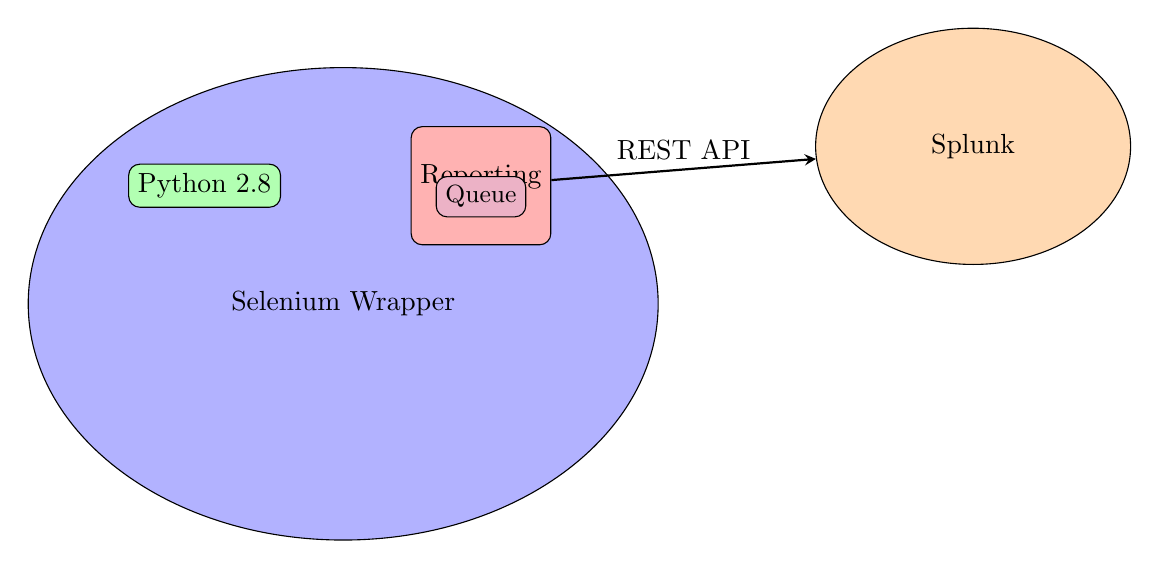
\begin{tikzpicture}

  \tikzstyle{startstop} = [rectangle, rounded corners, minimum width=3cm, minimum height=1cm,text centered, draw=black, fill=red!30]
  \tikzstyle{process} = [rectangle, minimum width=3cm, minimum height=1cm, text centered, draw=black, fill=orange!30]
  \tikzstyle{decision} = [diamond, minimum width=3cm, minimum height=1cm, text centered, draw=black, fill=green!30]

  \tikzstyle{external} = [rectangle, rounded corners, text centered, draw=black, fill=orange!30]
  \tikzstyle{internal} = [rectangle, rounded corners, text centered, draw=black, fill=red!30]
  \tikzstyle{q} = [internal, fill=purple!30]

  \tikzstyle{arrow} = [thick,->,>=stealth]

  \node (wrapper) [ellipse, minimum width=8cm, minimum height=6cm, text centered, draw=black, fill=blue!30] {Selenium Wrapper};
  \node (python)  [external, fill=green!30, yshift=1.5cm, xshift=-1.76cm] {Python 2.8}; 
  \node (report)  [internal, minimum height=1.5cm, yshift=1.5cm, xshift=1.75cm, text height=-0.75cm] {Reporting}; 
  \node (reportqueue) [q, minimum height=0.5cm, below of=report, yshift=0.86cm] {\small Queue};
  
  \node (splunk) [external, right of=wrapper, ellipse, xshift=7cm, yshift=2cm, minimum width=4cm, minimum height=3cm] {Splunk};
  \draw [arrow] (report) -- node[anchor=south] {REST API} (splunk);
















\end{tikzpicture}
\end{document}
